\documentclass[11pt,a4paper]{article}

\usepackage[T1]{fontenc}
\usepackage[utf8]{inputenc}
\usepackage[spanish]{babel}
\addto\captionsspanish{\renewcommand{\tablename}{Tabla}}
\usepackage{amsmath}
\usepackage{graphicx}
\usepackage{booktabs}
\usepackage{caption}
\usepackage[margin=2.5cm]{geometry}
\usepackage[colorlinks=true,linkcolor=black,citecolor=black,urlcolor=blue]{hyperref}

% La figura se busca en la carpeta del proyecto (Overleaf) o en ../figures (repositorio)
\graphicspath{{./}{../figures/}{../data/}}

\emergencystretch=2em

\title{Comparación carga--deflexión de una viga simplemente apoyada con la predicción de Euler--Bernoulli}
\author{Marcelo Palma Meléndez\\
\small Herramientas Computacionales 2 --- Hito 1}
\date{\today}

\begin{document}
\maketitle

\section{Problema y objetivo}
Se estudia una viga simplemente apoyada de sección rectangular, con una carga puntual aplicada en el centro de la luz (Figura~\ref{fig:esquema}). Se dispone de nueve pares carga--deflexión medidos en el centro de la luz. El objetivo es comparar la deflexión medida con la deflexión teórica de Euler--Bernoulli y evaluar si el modelo lineal elástico describe adecuadamente los datos.

\section{Datos y supuestos}
Los datos provienen de los archivos \texttt{datos\_viga.csv} (cargas de 0 a 40~kN y deflexión medida en mm) y \texttt{parametros\_viga.xlsx}. Los datos de deflexión son sintéticos y se entregaron solo con fines docentes. Los parámetros del caso se resumen en la Tabla~\ref{tab:param}.

\begin{table}[h]
\centering
\caption{Parámetros del caso.}
\label{tab:param}
\begin{tabular}{lcc}
\toprule
Parámetro & Valor & Unidad \\
\midrule
Luz entre apoyos, $L$ & $4$ & m \\
Ancho de la sección, $b$ & $0{,}2$ & m \\
Altura de la sección, $h$ & $0{,}4$ & m \\
Módulo de elasticidad, $E$ & $25$ & GPa \\
\bottomrule
\end{tabular}
\end{table}

\begin{figure}[h]
\centering
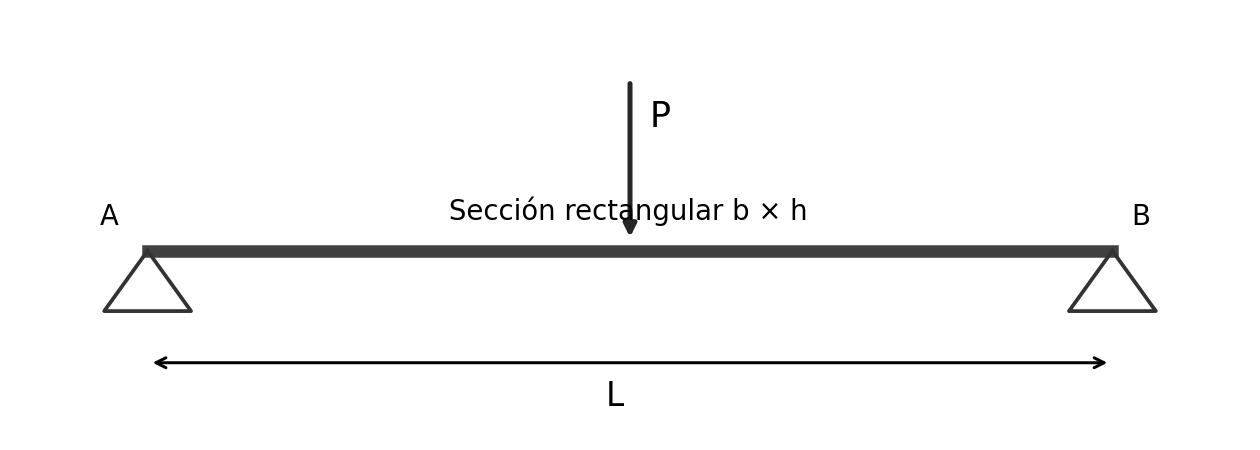
\includegraphics[width=0.5\textwidth]{esquema_viga.png}
\caption{Esquema de la viga simplemente apoyada con carga puntual centrada.}
\label{fig:esquema}
\end{figure}

Se supone un material homogéneo, isótropo y linealmente elástico, pequeñas deflexiones, apoyos simples ideales y carga puntual exactamente centrada. Siguiendo la teoría de Euler--Bernoulli se desprecian la deformación por corte y el peso propio.

\section{Método}
El segundo momento de área de la sección rectangular es
\begin{equation}
I = \frac{b\,h^{3}}{12}.
\label{eq:I}
\end{equation}
Para una carga puntual $P$ en el centro de una viga simplemente apoyada, la deflexión teórica en el centro es \cite[Ap.~C, p.~814]{hibbeler}
\begin{equation}
\delta_{\mathrm{teo}} = \frac{P\,L^{3}}{48\,E\,I}.
\label{eq:delta}
\end{equation}
Para las cargas distintas de cero se calcula la diferencia relativa
\begin{equation}
\varepsilon = \frac{\delta_{\mathrm{med}}-\delta_{\mathrm{teo}}}{\delta_{\mathrm{teo}}}.
\label{eq:eps}
\end{equation}

Para obtener $\delta_{\mathrm{teo}}$ en metros, los datos se llevaron al Sistema Internacional: $1\ \mathrm{kN}=1000\ \mathrm{N}$ y $1\ \mathrm{GPa}=10^{9}\ \mathrm{Pa}$. El resultado se convirtió a milímetros ($1\ \mathrm{m}=1000\ \mathrm{mm}$) para compararlo con la deflexión medida, que se mantuvo en mm. Con los datos del caso, $I = 1{,}0667\times10^{-3}\ \mathrm{m^{4}}$ y la deflexión teórica por unidad de carga es $0{,}05\ \mathrm{mm/kN}$.

Los cálculos se realizaron en una planilla (\texttt{analysis/analisis\_viga.xlsx}) donde cada columna es una fórmula que referencia las celdas de parámetros, de modo que el cálculo es rastreable. Los archivos originales se conservaron sin modificar y el trabajo se organizó en un repositorio con control de versiones: \url{https://github.com/marcelopalmam-jpg/hito-1-viga-}.

\section{Resultados y verificación}
La Tabla~\ref{tab:res} compara la deflexión medida con la teórica, y la Figura~\ref{fig:cd} muestra ambas series.

\begin{table}[h]
\centering
\caption{Deflexión medida y teórica en el centro de la luz.}
\label{tab:res}
\begin{tabular}{cccc}
\toprule
$P$ (kN) & $\delta_{\mathrm{med}}$ (mm) & $\delta_{\mathrm{teo}}$ (mm) & $\varepsilon$ (\%) \\
\midrule
5  & 0,26 & 0,25 & 4,00 \\
10 & 0,50 & 0,50 & 0,00 \\
15 & 0,76 & 0,75 & 1,33 \\
20 & 1,01 & 1,00 & 1,00 \\
25 & 1,28 & 1,25 & 2,40 \\
30 & 1,54 & 1,50 & 2,67 \\
35 & 1,77 & 1,75 & 1,14 \\
40 & 2,05 & 2,00 & 2,50 \\
\bottomrule
\end{tabular}
\end{table}

\begin{figure}[h]
\centering
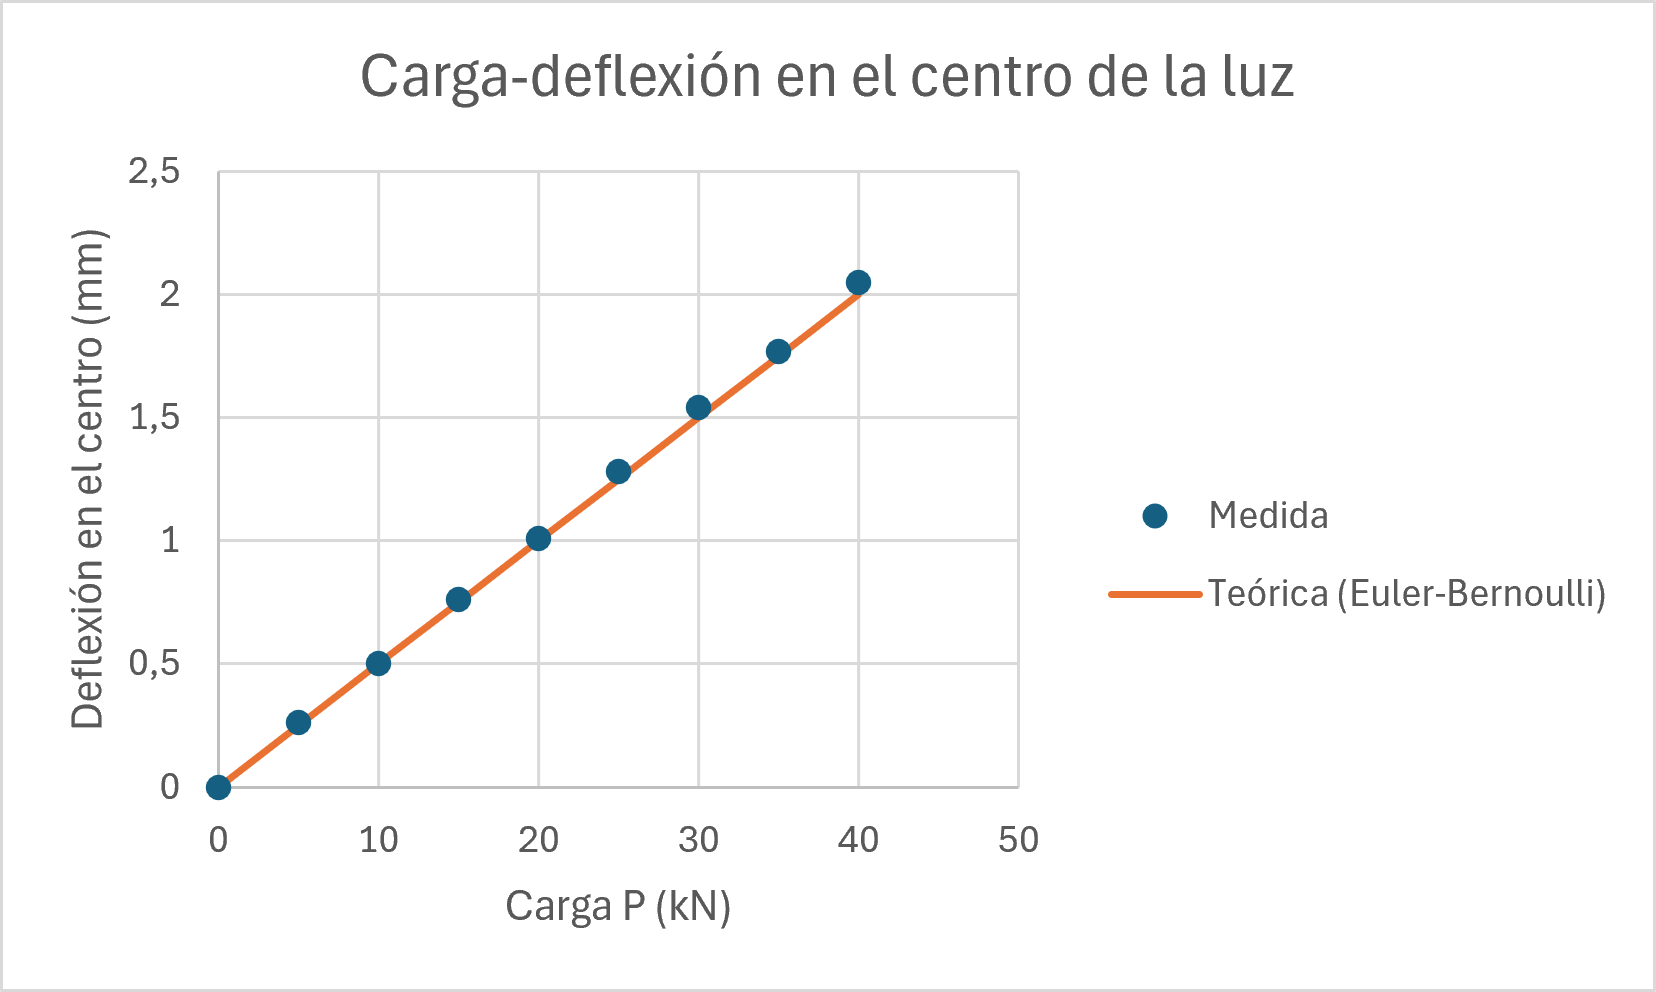
\includegraphics[width=0.65\textwidth]{carga_deflexion.png}
\caption{Deflexión en el centro de la luz en función de la carga: datos medidos (puntos) y predicción teórica de Euler--Bernoulli (línea).}
\label{fig:cd}
\end{figure}

La diferencia relativa varía entre 0,0\,\% y 4,0\,\%, con un promedio de 1,9\,\%, y la deflexión medida resulta siempre igual o ligeramente mayor que la teórica.

Se realizaron dos verificaciones adicionales:
\begin{enumerate}
\item \emph{Constancia de $\delta/P$.} En el rango lineal la relación $\delta_{\mathrm{med}}/P$ debe ser aproximadamente constante. Los valores medidos están entre $0{,}0500$ y $0{,}0520\ \mathrm{mm/kN}$, con promedio $0{,}0509\ \mathrm{mm/kN}$, frente a $0{,}0500\ \mathrm{mm/kN}$ de la predicción teórica (diferencia de 1,9\,\%).
\item \emph{Cálculo independiente de una fila.} Para $P=20\ \mathrm{kN}$, con el cálculo manual
\[
\delta = \frac{20\,000\cdot 4^{3}}{48\cdot 25\times10^{9}\cdot 1{,}0667\times10^{-3}} = 1{,}00\ \mathrm{mm},
\]
que coincide con el valor de la planilla.
\end{enumerate}

\section{Interpretación y conclusiones}
Los datos se comportan de forma lineal: la deflexión aumenta en proporción a la carga, y la fórmula de Euler--Bernoulli se acerca bastante a lo medido. La diferencia relativa llega como máximo a 4\,\% y en promedio es de 1,9\,\%. La diferencia más grande aparece con la carga más baja (5~kN), pero en ese caso equivale a solo 0,01~mm, que es el último decimal con que se reportan las mediciones. Por eso no la considero significativa por sí sola.

En casi todas las cargas la deflexión medida resultó un poco mayor que la teórica. Esto podría deberse a cosas que la fórmula no considera, como la deformación por corte, que los apoyos no sean perfectamente rígidos o que el módulo de elasticidad real sea algo menor que el usado. Con estos datos no puedo saber cuál de esas causas es la correcta, así que son solo posibles explicaciones.

El análisis tiene varias limitaciones. Los datos son sintéticos y corresponden a un solo ensayo, sin repeticiones, por lo que no se puede estimar la incertidumbre de la medición. Solo hay ocho cargas distintas de cero y un único conjunto de parámetros. Además, el módulo de elasticidad viene dado y no fue medido. El modelo tampoco incluye el corte ni el peso propio de la viga, y hasta 40~kN no se alcanza a ver comportamiento no lineal. En resumen, en el rango estudiado el modelo lineal elástico sirve para predecir la deflexión en el centro de la viga.
\section*{Declaración de uso de inteligencia artificial}
Usé Claude como apoyo durante todo el trabajo. Me ayudó a entender los pasos de la actividad, a revisar mis cálculos y fórmulas, y a organizar el repositorio y la planilla. También me hizo la estructura de la nota en LaTeX y un borrador del texto, que después revisé y modifiqué con mis propias palabras. Los cálculos los hice yo en la planilla y los verifiqué con un cálculo manual independiente. Además, revisé yo mismo la fórmula de la deflexión máxima en la tabla de deflexiones de vigas de Hibbeler~\cite[Ap.~C, p.~814]{hibbeler}. Soy responsable del contenido entregado y puedo explicarlo. Más detalle en el archivo \texttt{USO\_IA.md} del repositorio.
\bibliographystyle{plain}
\bibliography{referencias}

\end{document}
